\clearpage{\pagestyle{empty}\cleardoublepage}

\chapter{Sistemi di piggaggio di condotte in pressione}\thispagestyle{empty} 
\chaptermark{Piggaggio}
Il piggaggio, detto anche \textit{pigging}, è un'applicazione nella quale un dispositivo cilindrico o sferico chiamato scovolo (o \textit{pig}), opportunamente dimensionato, viene spinto all'interno di una condotta tramite variazioni indotte di pressione e flusso del mezzo presente all'interno, tramite l'introduzione di un mezzo esterno o tramite movimento meccanico. Lo scovolo viene immesso in condotta al fine di pulire, ispezionare, dosare inibitori chimici lungo la tubazione oppure isolare delle sezioni specifiche della rete.\\
L'origine del termine inglese \textit{pig} è tuttora incerto: se da una parte viene proposto come l'acronimo di \textit{Pipeline Intervention Gadget}, dall'altra si fa riferimento al rumore che provoca lo scorrimento dello scovolo in condotta, simile al verso di un maiale \parencite{varghese2011intelligent}.\\
Durante gli anni '40 negli Stati Uniti il piggaggio aveva come fine principale la rimozione di paraffina per migliorare l'efficienza delle condotte a olio, quindi veniva usato per aumentare la produzione e sopperire all'alta domanda legata alle attività belliche della Seconda Guerra Mondiale.\\
Nel mondo oggi il piggaggio è impiegato per numerosi scopi e la strumentazione  è progettata dagli ingegneri in base alle necessità legate all'applicazione.\\
Il seguente capitolo offre una panoramica riguardo al piggaggio delle condotte in pressione dove vengono mostrate le varie configurazioni degli scovoli, le finalità dell'applicazione, le procedure operative e la valutazione di soluzioni in caso di blocco del \textit{pig} in linea.

\section{Configurazione degli scovoli}
L'assemblaggio e configurazione dello scovolo di servizio prevede numerose soluzioni:
\begin{itemize}
	\item \textbf{a mandrino} (\figref{fig:mandrel}): gli elementi dello scovolo sono assemblati sul corpo centrale tramite numerosi bulloni;
	\item \textbf{a bullone singolo} (\figref{fig:singlebolt}): simile allo scovolo a mandrino, gli accessori del \textit{pig} in questo caso sono inseriti tramite un'unica bullonatura longitudinale;
	\item \textbf{a telaio fisso} (\figref{fig:solidcast}): sia le tenute che gli elementi guida sono rivestiti da un corpo unico di poliuretano;
	\item \textbf{a schiuma} (\figref{fig:foampig}): solitamente con struttura aperta di poliuretano, questi scovoli sono disponibili a diversa densità, a seconda dell'applicazione richiesta. Il rivestimento aumenta la resistenza a usura e la stabilità dell'utensile;
	\item \textbf{sfere} (\figref{fig:spherepig}): possono essere piene o riempite con aria, acqua o glicol, possono essere usate come tamponi o rimozione liquidi;
	\item \textbf{articolato} (\figref{fig:articulated}): composto da due o più scovoli uniti tra loro con sistemi di accoppiamento universale. Rappresenta la configurazione base degli scovoli intelligenti;

\end{itemize}

\begin{figure}[htbp]
    \centering
    \subfloat[][A mandrino.]
    {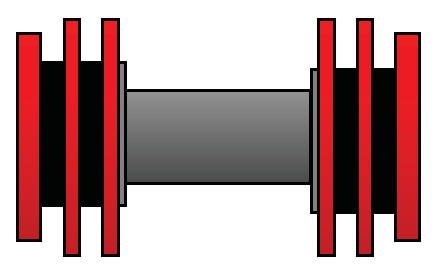
\includegraphics[height=.1\textheight]{fig/pig/configurazione/mandrel.eps}  \label{fig:mandrel}} \qquad
    \subfloat[][A bullone singolo.]
    {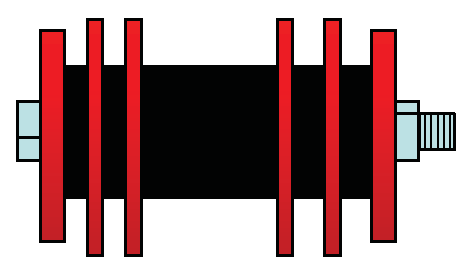
\includegraphics[height=.1\textheight]{fig/pig/configurazione/singlebolt.eps}  \label{fig:singlebolt}} \qquad 
    \subfloat[][A telaio fisso.]
    {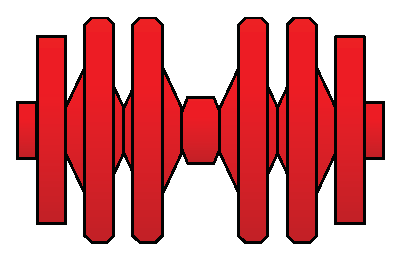
\includegraphics[height=.1\textheight]{fig/pig/configurazione/solidcast.eps}  \label{fig:solidcast}} \\
    \subfloat[][A schuma.]
    {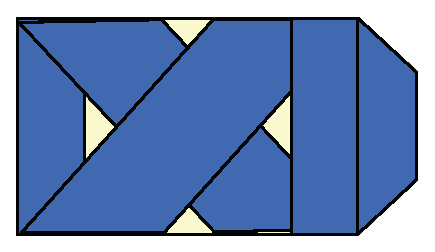
\includegraphics[height=.1\textheight]{fig/pig/configurazione/foam.eps}  \label{fig:foampig}} \qquad
    \subfloat[][Sfere.]
    {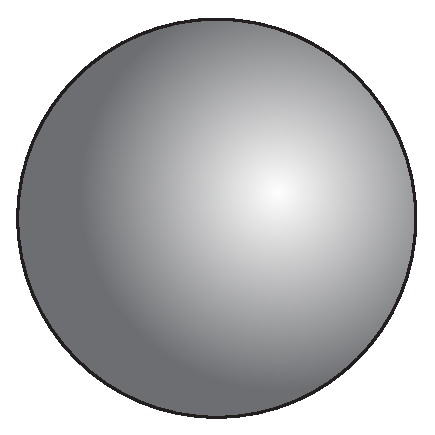
\includegraphics[height=.1\textheight]{fig/pig/configurazione/sphere.eps}  \label{fig:spherepig}} \\
    \subfloat[][Articolato.]
    {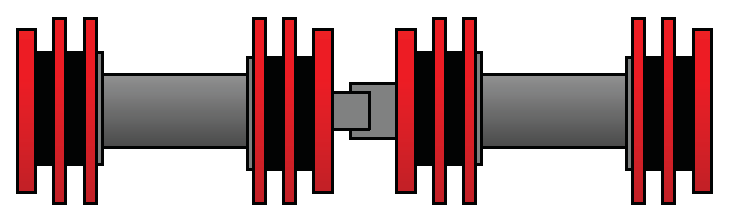
\includegraphics[height=.1\textheight]{fig/pig/configurazione/articulated.eps}  \label{fig:articulated}}
\caption{Configurazione dello scovolo \parencite{davidson2002introduction}.}
\label{fig:configurazione}
\end{figure}

Gli scovoli a mandrino e a bullone singolo si adattano alla richiesta specifica grazie all'installazione di diversi dispositivi sul corpo centrale.\\
e spazzole (\figref{fig:spazzole}) sono impiegate in primo luogo per la rimozione di depositi compatti come calcare e prodotti da corrosione. Alcune spazzole sono specifiche per favorire l'azione degli inibitori di corrosione e dei biocidi in condotta.\\
Le guarnizioni a tazza (\figref{fig:tazze}) sono dispositivi di tenuta idraulica che consentono lo spostamento unidirezionale dello scovolo attraverso la spinta di un fluido da monte. Sono utilizzati anche come dispositivi di \textit{batching}. Le coppelle coniche rappresentano una valida alternativa alle guarnizioni a tazza, differiscono da quest'ultime per la convessità della tenuta rispetto alla parete della condotta.\\
I dischi (\figref{fig:dischi}) vengono utilizzati come tenute idrauliche, per la pulizia e come organi di supporto. A differenza delle guarnizioni a tazza e le coppelle coniche, uno scovolo dotato di dischi può muoversi in entrambe le direzioni.\\
Le lame (\figref{fig:lame}), tramite l'azione di taglio, provvedono alla rimozione di depositi morbidi come paraffina e fanghi, vengono quindi impiegate in condotte dedicate al trasporto di olio.\\
L'inserimento di potenti magneti (\figref{fig:magneti}) sulla circonferenza permette allo scovolo non solo l'asportazione di materiale ferroso dalla condotta, ma anche di attivare i segnalatori posti all'esterno della condotta per monitorarne il tragitto.\\
Lo scovolo può essere dotato inoltre di accessori per la misurazione: possono essere di varia natura (calibri, dischi misuratori, dispositivi magnetici, etc.) e consentono l'ispezione interna della condotta.
%I singolo dispositivi possono essere accoppiati sullo stesso dispositivo, al fine di sopperire a più richieste con un unico passaggio dello scovolo in condotta (\figref{fig:assemblato}).


\begin{figure}[htbp]
    \centering
    \subfloat[][Scovolo con spazzole a molla.]
    {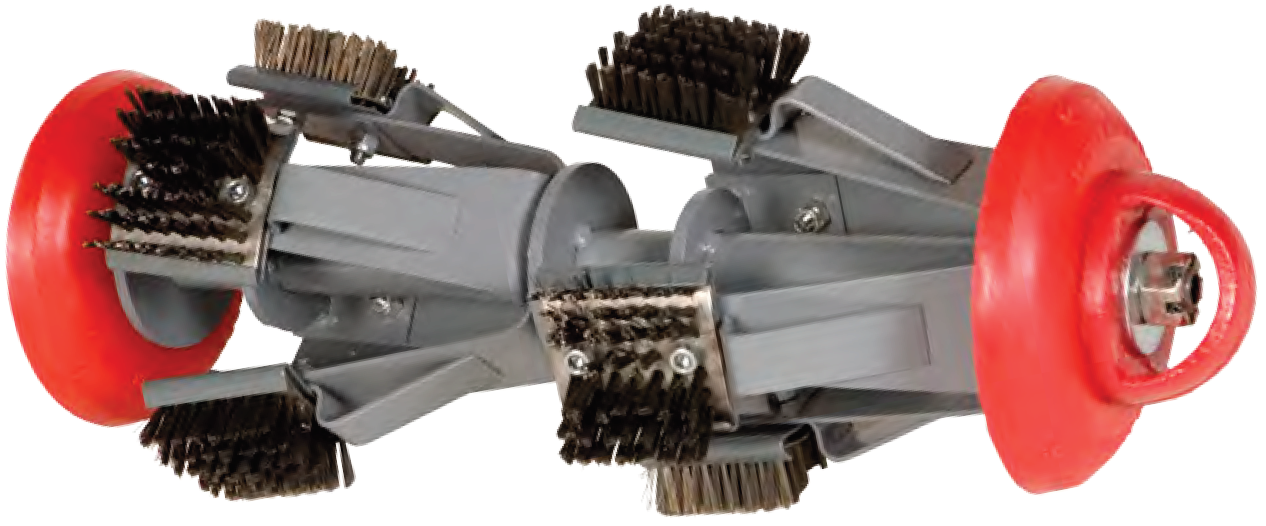
\includegraphics[height=.12\textheight]{fig/pig/tool/spazzolemolla}  \label{fig:spazzole}} \qquad
    \subfloat[][Scovolo con guarnizioni a tazza.]
    {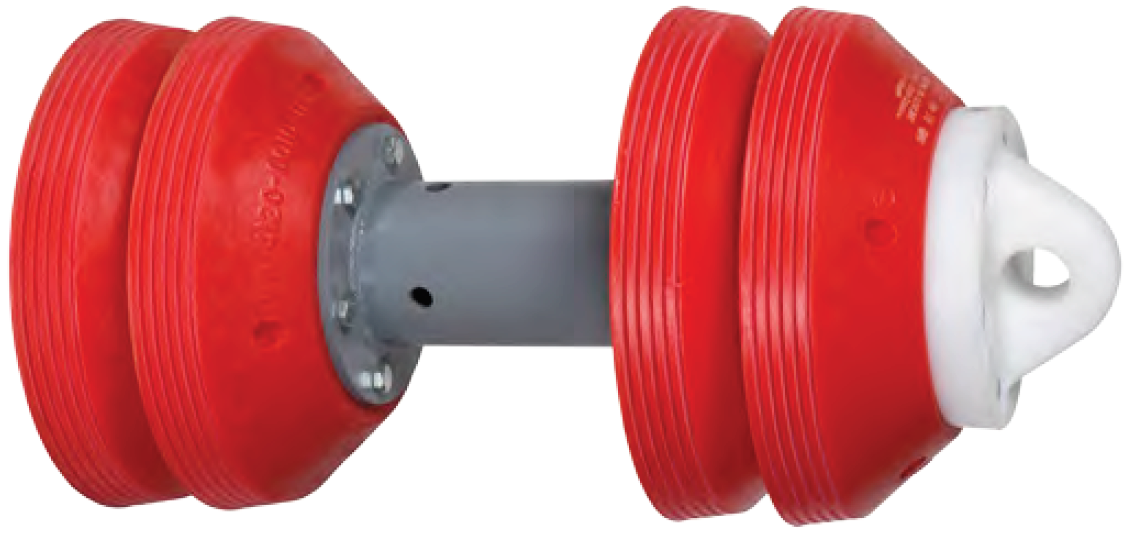
\includegraphics[height=.12\textheight]{fig/pig/tool/tazze}  \label{fig:tazze}} \qquad
    \subfloat[][Scovolo con dischi.]
    {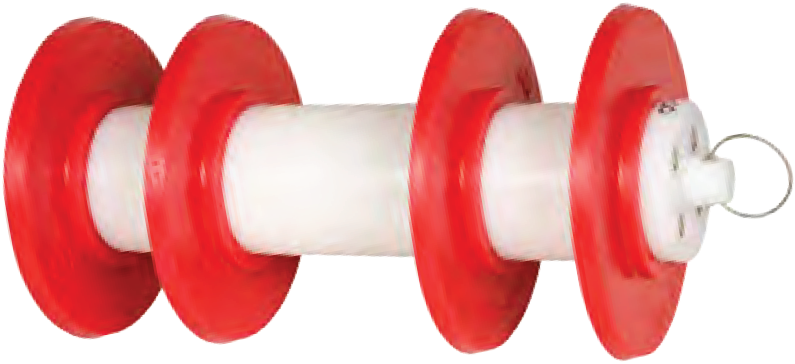
\includegraphics[height=.12\textheight]{fig/pig/tool/dischi}  \label{fig:dischi}} \\
    \subfloat[][Scovolo con lame di poliuretano.]
    {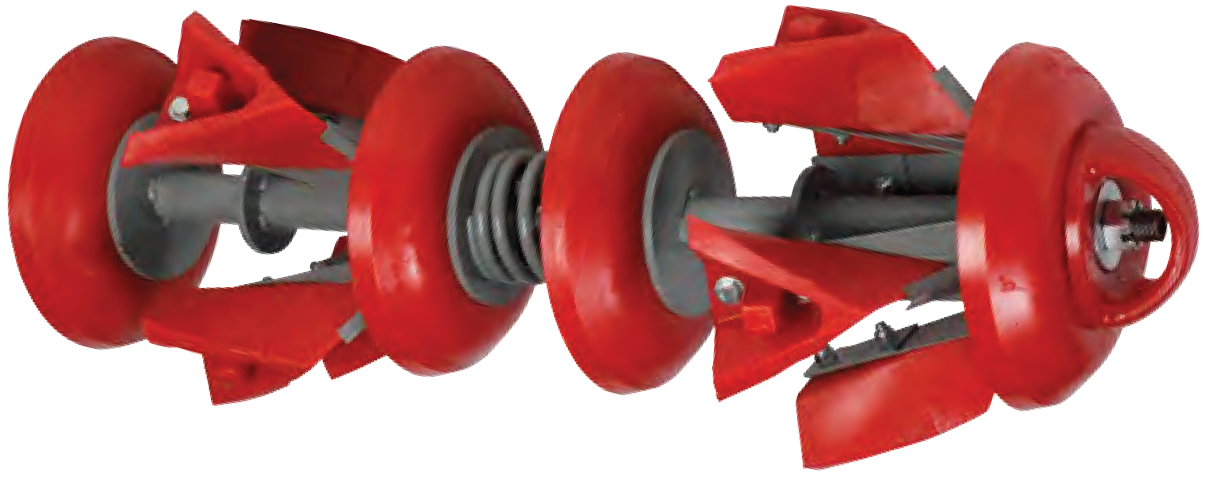
\includegraphics[height=.12\textheight]{fig/pig/tool/lame}  \label{fig:lame}} \qquad
    \subfloat[][Scovolo con magneti sulla circonferenza.]
    {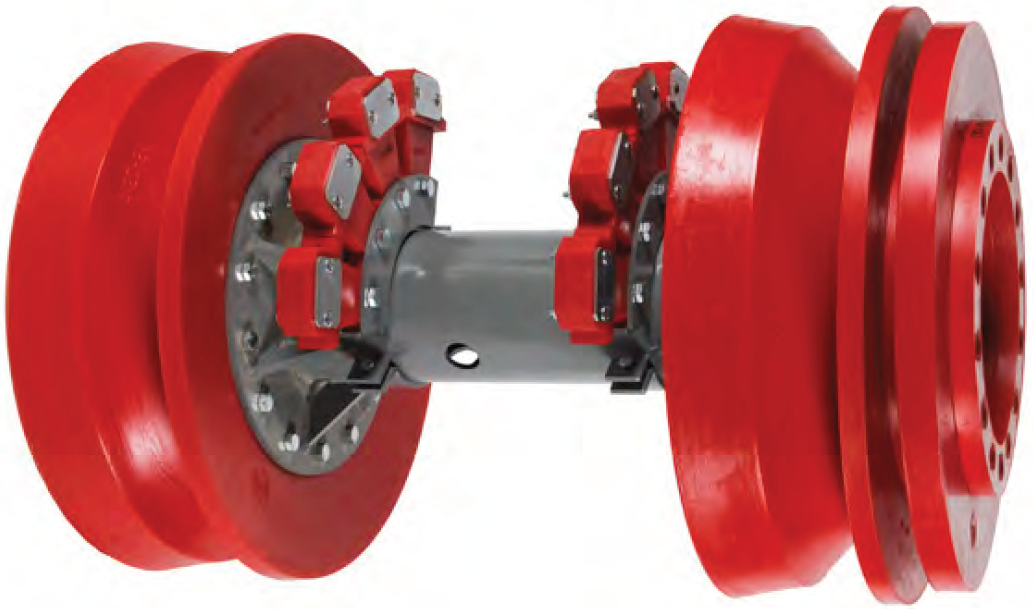
\includegraphics[height=.12\textheight]{fig/pig/tool/magneti}  \label{fig:magneti}} \qquad
%    \subfloat[][Scovolo con spazzole circolari, guarnizioni a tazza e dischi.]
%    {\includegraphics[height=.12\textheight]{fig/pig/tool/assemblato}  \label{fig:assemblato}}
\caption{Componenti tipici di uno scovolo di servizio \parencite{williamson2015guide}.}
\label{fig:dispositivi}
\end{figure}

\section{Obiettivi del piggaggio}
Il piggaggio di una condotta viene oggi eseguito in tutte le fasi di vita di un impianto di processo. Data la sua versatilità, è di consuetudine per tutti i settori dell'industria di processo, perciò non esistono delle classificazioni universali degli scovoli impiegati. Una generica distinzione tra \textit{pig} può essere fatta in base all'operazione richiesta: si parla quindi di scovoli di servizio, scovoli per l'ispezione interna e scovoli gel.

\subsection{Scovoli di servizio}
Qui di seguito sono elencati i motivi legati generalmente all'impiego di scovoli di servizio:
\begin{itemize}
	\item \textbf{pulizia della condotta}: utile per migliorare le condizioni di flusso;
	\item \textbf{separazione dei fluidi} o \textit{\textbf{batching}}: scovoli di separazione tra diversi prodotti chimici da applicare in condotta;
%		\item \textbf{ispezione interna}: è importante monitorare le condizioni interne della condotta, così da prevedere eventuali rotture o imprevisti di produzione. Gli scovoli possono assumere numerose configurazioni (forma e dimensioni), obiettivo ultimo è il rilevamento di ammaccature, consumo interno della parete interna e crepe.
	\item \textbf{spiazzamento della condotta}: specialmente nelle condotte a gas, gli scovoli possono essere utilizzati per spiazzare delle formazioni liquide indesiderate in condotta.
\end{itemize}

\subsubsection{Pulizia}
Gli scovoli pulenti sono impiegati per mantenere dei livelli di efficienza minimi in condotta. Nel settore degli idrocarburi, qualunque riduzione di portata corrisponde a un mancato introito giornaliero. La riduzione della portata è legata all'attrito e a fattori fisici. Nelle condotte a gas i problemi di produzione sono legati alla presenza di elementi corrosivi, detriti e depositi, polveri e condensati. Nel caso del greggio le condotte risentono della presenza di sabbia e paraffina adesa alle pareti interne della tubazione.\\
Si valuta l'efficienza di una condotta tramite considerazioni tecniche su flusso, cadute di pressione e costi operativi. Nel momento in cui la condotta necessita di una pulizia interna, si inserisce uno scovolo lungo il tratto interessato.\\
\begin{figure}[htbp]
	\centering
	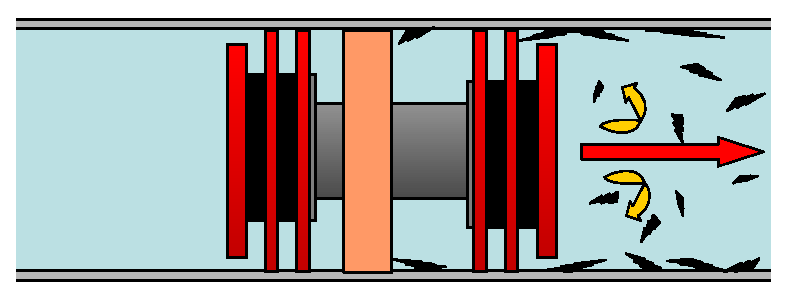
\includegraphics[width=.7\textwidth]{fig/pig/cleaning.eps}
	\label{fig:cleaningpig}
	\caption{Scorrimento dello scovolo di pulizia in condotta e rimozione dei depositi solidi in condotta \parencite{davidson2002introduction}.}
\end{figure}
La configurazione migliore del \textit{pig} pulente consiste in dischi, guarnizioni a tazza e dispositivi pulenti rappresentati da spazzole radiali a molla o lame in poliuretano (\figref{fig:assemblato}). I dischi consentono di spingere via i residui solidi oltre a fornire un buon supporto, guarnizioni provvedono alla tenuta. Le spazzole consentono la rimozione di ruggine, detriti e altri residui solidi; le lame sono impiegate in condotte a olio, grazie alla maggiore efficacia sulla paraffina e la facilità di pulizia al termine dell'applicazione (\figref{fig:paraffina}). \\
Nella pulizia di condotte con mezzi liquidi gli scovoli possono essere dotati di \textit{bypass} (\figref{fig:bypass}), ugelli longitudinali che convogliano del liquido in pressione da monte a valle, evitando così il deposito dei solidi sul fondo e riducendo la velocità di scorrimento del dispositivo.\\
Gli scovoli di pulizia tradizionali non agiscono propriamente sul materiale metallico come aste, bulloni o utensili lasciati dopo la messa in opera della condotta. Il modo più efficace consiste nell'installazione di nastri magnetici lungo il corpo dello scovolo (\figref{fig:magnetipulizia}). 

\begin{figure}[htbp]
    \centering
    \subfloat[][Scovolo con spazzole circolari, guarnizioni a tazza e dischi.]
    {\makebox[0.45\textwidth]{\includegraphics[height=.12\textheight]{fig/pig/cleaning/assemblato}}  \label{fig:assemblato}}\qquad
    \subfloat[][Scovolo a lame con paraffina adesa.]
    {\makebox[0.45\textwidth]{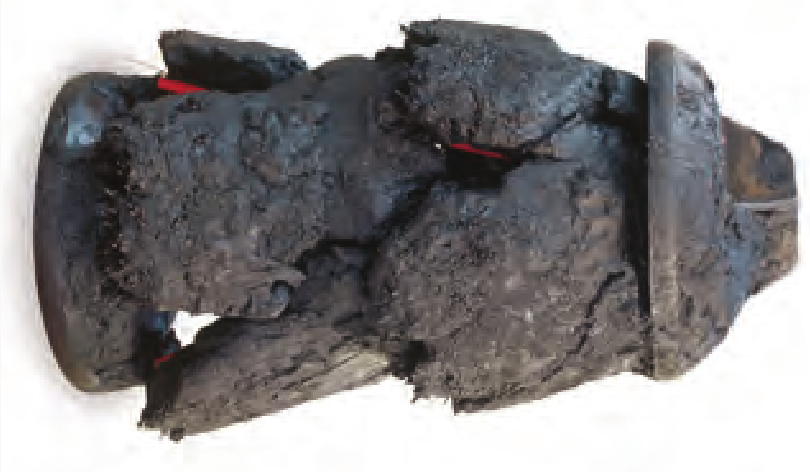
\includegraphics[height=.12\textheight]{fig/pig/cleaning/paraffina}}  \label{fig:paraffina}}\\
    \subfloat[][Ugelli di \textit{bypass}.]
    {\makebox[0.45\textwidth]{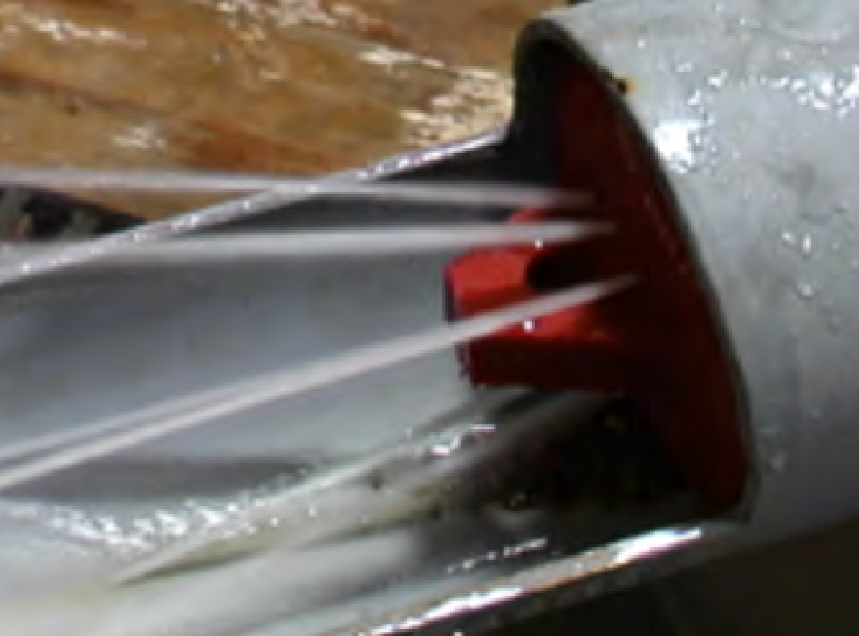
\includegraphics[height=.12\textheight]{fig/pig/cleaning/bypass}}  \label{fig:bypass}}\qquad
    \subfloat[][Scovolo per la pulizia dei residui metallici.]
    {\makebox[0.45\textwidth]{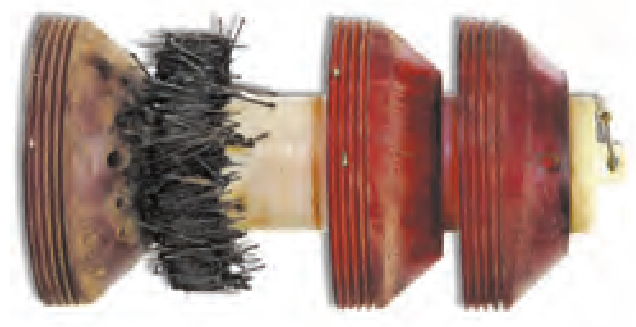
\includegraphics[height=.12\textheight]{fig/pig/cleaning/magnetipulizia}}  \label{fig:magnetipulizia}}
\caption{Dispositivi di pulizia delle condotte \parencite{williamson2015guide}.}
\label{fig:dispositivipulizia}
\end{figure}

\subsubsection{Spiazzamento}
Per spiazzamento della condotta si intende la completa sostituzione di un mezzo fluido con un altro. Gli scovoli di spiazzamento o separazione, tramite meccanismi di spinta e di tenuta, consentono di effettuare queste operazioni. Numerose sono le operazioni che necessitano l'impiego di questi dispositivi.\\
I test di tenuta idraulica di una condotta prevedono lo spurgo totale, il riempimento con acqua e la pressurizzazione della linea per un determinato periodo di tempo tramite scovoli di spiazzamento. Altri impieghi sono la separazione tra idrocarburi e gas inerte per poter effettuare riparazioni sul campo o lo spiazzamento di liquidi indesiderati da linee a gas.\\
La configurazione generica è rappresentata dagli scovoli a quattro tazze di tenuta, tenute in contatto con le pareti della condotta. Per ovviare alle variazioni di diametro interno, si utilizzano delle guarnizioni a tazza a più labbra di tenuta (\textit{multi-lipped cup}, \figref{fig:displacement-multilipped}).\\
Gli scovoli a dischi bidirezionali (\figref{fig:displacement-bidirezionale}) sono tipicamente usati nelle operazioni di riempimento e spiazzamento acqua in condotta, associati quindi ai test di tenuta. La possibilità di agire in direzione doppia consente la ricollocazione del dispositivo in posizione iniziale nel caso in cui si preveda un possibile blocco in condotta.\\
Le sfere (\figref{fig:displacement-unisphere}) sono la soluzione ideale per la rimozione di liquidi da linee a gas. I sistemi di piggaggio a sfere sono progettati per il lancio e la ricezione in automatico, con un numero di sfere che può variare in base alle richieste specifiche. Sul punto di ricezione, si prevede l'installazione di uno \textit{slug catcher} per ovviare al volume di liquido associato alle sfere. Le condotte a gas sono normalmente progettate per l'uso di sfere ma ciò non vuol dire che possano essere piggabili da scovoli convenzionali.\\
Schiume a bassa densità senza rivestimento (\figref{fig:displacement-schiuma}) sono impiegate per asciugare la condotta dopo l'operazione di spiazzamento d'acqua. Questi \textit{pig} hanno come unico svantaggio la possibilità di potersi bloccare in opera.\\
 
\begin{figure}[htbp]
    \centering
    \subfloat[][Guarnizione a tazza a più labbra di tenuta.]
    {\makebox[0.45\textwidth]{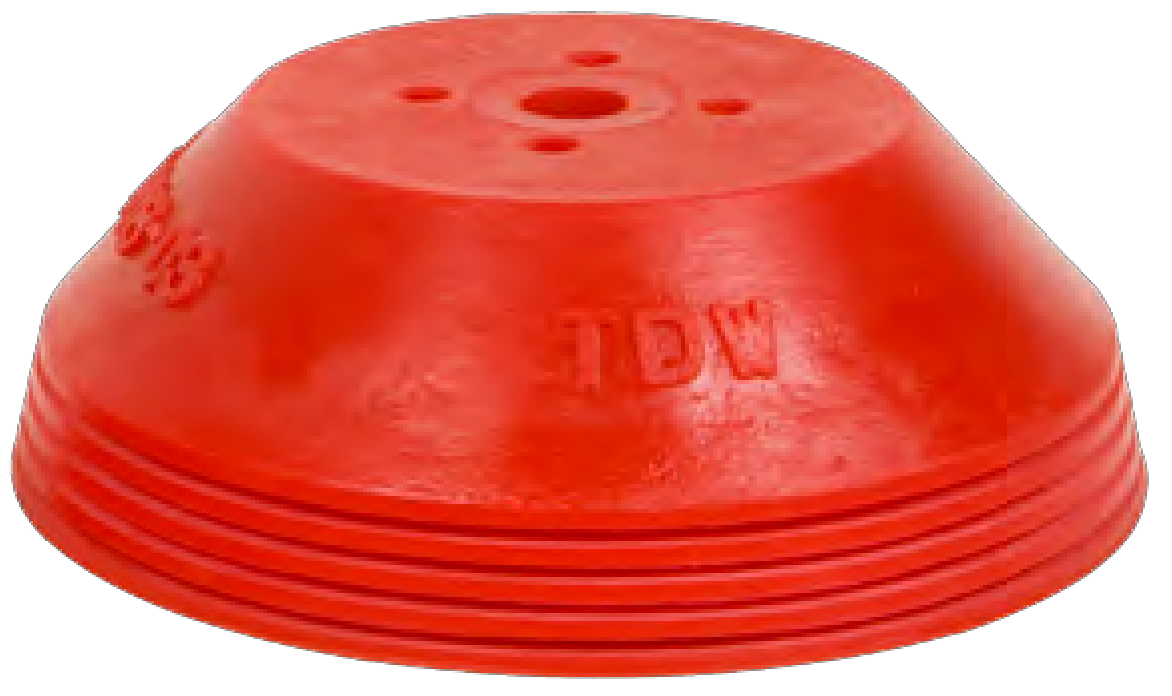
\includegraphics[height=.12\textheight]{fig/pig/displacement/multilipped}}  \label{fig:displacement-multilipped}}\qquad
    \subfloat[][Scovolo a dischi bidirezionale.]
    {\makebox[0.45\textwidth]{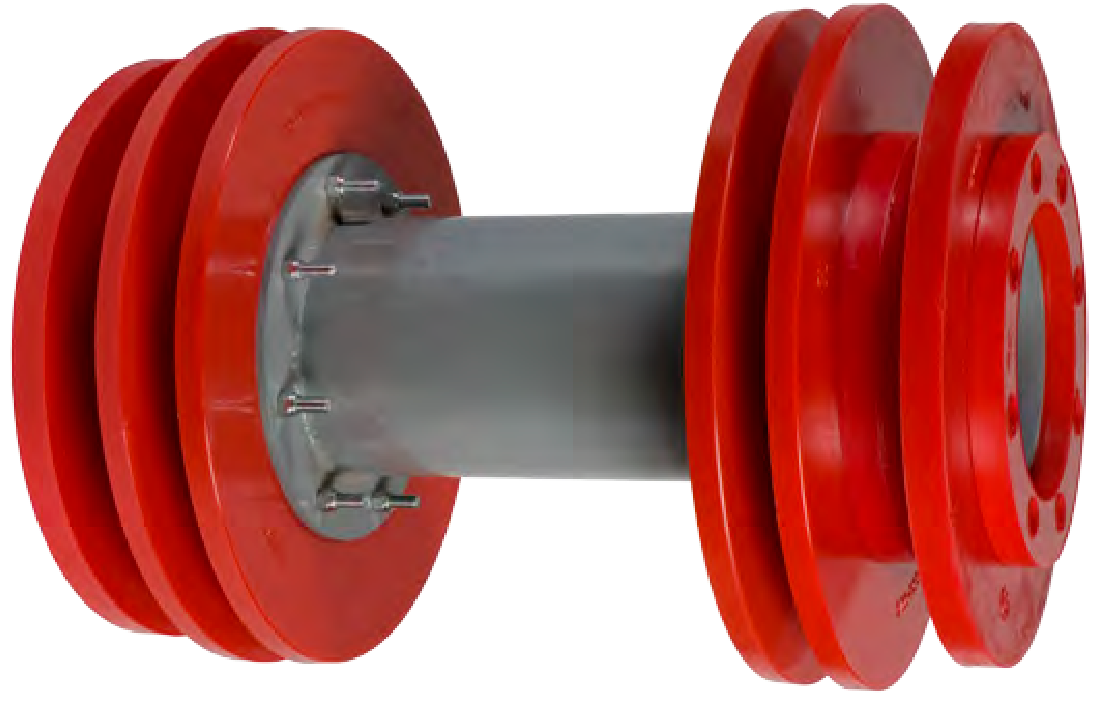
\includegraphics[height=.12\textheight]{fig/pig/displacement/bidirezionale}}  \label{fig:displacement-bidirezionale}}\\
    \subfloat[][Sfere UNISPHERE™.]
    {\makebox[0.45\textwidth]{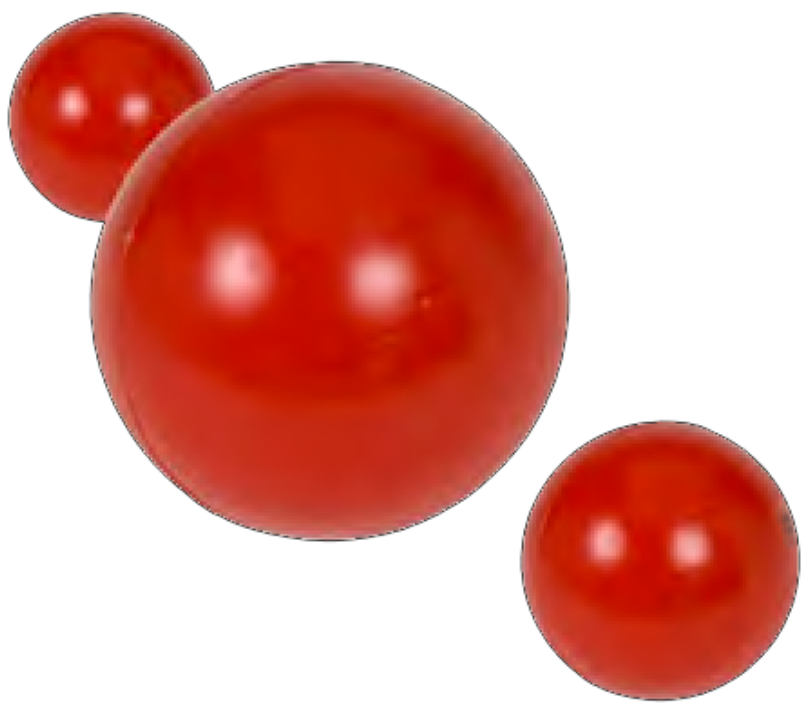
\includegraphics[height=.12\textheight]{fig/pig/displacement/unisphere}}  \label{fig:displacement-unisphere}}\qquad
    \subfloat[][Scovoli a schiuma senza rivestimento a bassa densità.]
    {\makebox[0.45\textwidth]{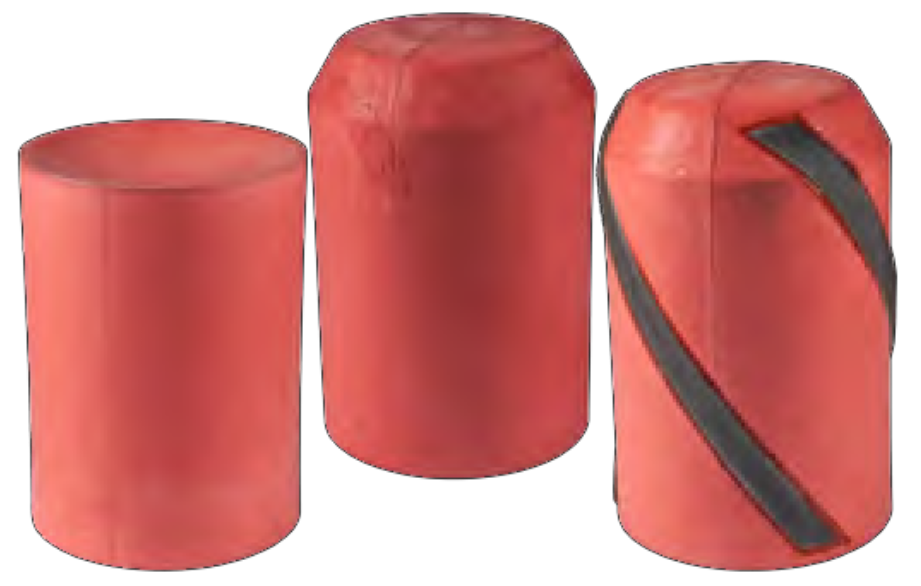
\includegraphics[height=.12\textheight]{fig/pig/displacement/schiuma-norivestimento}}  \label{fig:displacement-schiuma}}
\caption{Diverse tipologie di trappole di lancio \parencite{williamson2015guide}.}
\label{fig:displacement-tools}
\end{figure} 
 
\subsubsection{Separazione dei fluidi}
In alcune applicazioni si richiede l'immissione di uno o più prodotti separatamente. Nella condotta si possono creare delle condizioni di "contaminazione" a causa di:
\begin{itemize}
	\item regime di flusso;
	\item geometria della condotta;
	\item procedure operative.
\end{itemize}
Al fine di ovviare al contatto tra i diversi prodotti, si impiegano in condotta degli scovoli tampone o \textit{batching pig}, dispositivi di tenuta idraulica in grado di evitare il contatto tra i singoli \textit{slug}. La \figref{fig:batching} mostra un'applicazione tipica: i primi due \textit{slug} di acqua dolce provvedono alla desalinizzazione della linea precedentemente percorsa dall'acqua di mare, mentre gli \textit{slug} di glicol permettono la deidratazione e l'inibizione degli idrati.

\begin{figure}[htbp]
	\centering
	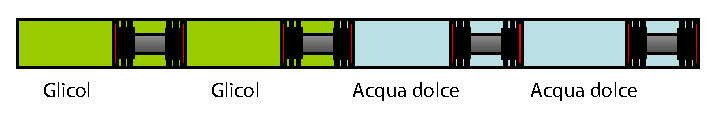
\includegraphics[width=\textwidth]{fig/pig/batching.eps}
	\caption{Desalinizzazione della condotta con treni di acqua dolce e glicol \parencite{davidson2002introduction}.}
	\label{fig:batching}
\end{figure}

Gli scovoli impiegati per la separazione di prodotti sono gli stessi usati per lo spiazzamento: in particolar modo si parla di guarnizioni a tazza, coppelle coniche e dischi bidirezionali.

\subsection{Strumenti di ispezione interna}
Questi dispositivi provvedono a fornire informazioni sulle condizioni della condotta, così come l'estensione e la localizzazione di qualsiasi problema presente. Gli scovoli di ispezione interna più semplice sono di misurazione meccanica.\\
Lo scovolo a piastra spessimetrica (\figref{fig:gauging}) è un dispositivo di misurazione molto semplice: lo strumento di misura consiste in un disco dal diametro pari al 95\% di quello della condotta interna. Associato a un emettitore acustico, lo scovolo emette un segnale quando si presenta un restringimento, fornendo quindi indicazioni agli operatori per la riparazione della condotta. \\
Lo scovolo calibro (\figref{fig:caliper}) è utile alla misurazione della geometria interna della condotta. Un sistema di leve metalliche radiali, in questo caso definito calibro, è collegato a un dispositivo di registrazione interno, il quale tiene traccia del profilo interno della condotta in funzione della posizione. 

\begin{figure}[htbp]
    \centering
    \subfloat[][Scovolo a piastra spessimetrica.]
    {\makebox[0.45\textwidth]{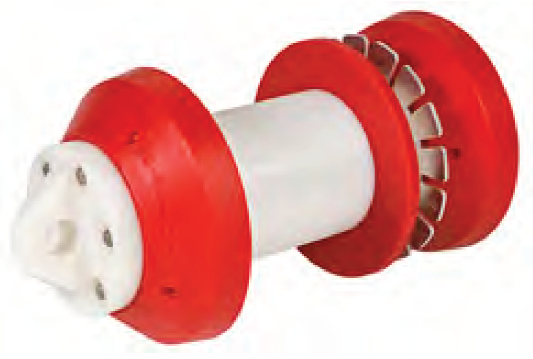
\includegraphics[height=.12\textheight]{fig/pig/gauging}}  \label{fig:gauging}} \qquad
    \subfloat[][Scovolo calibro.]
    {\makebox[0.45\textwidth]{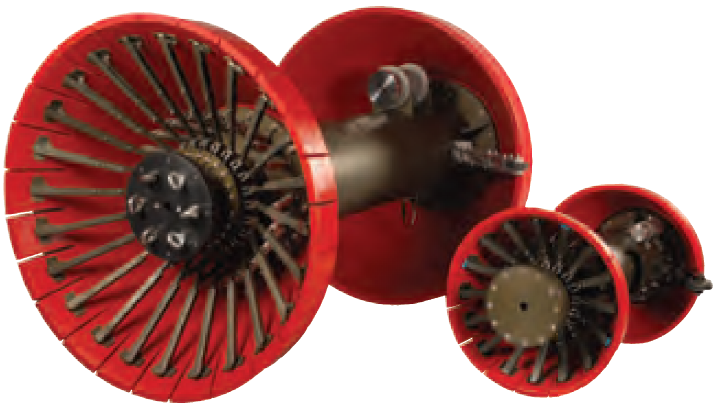
\includegraphics[height=.12\textheight]{fig/pig/caliper}}  \label{fig:caliper}}
\caption{Scovoli di ispezione interna tradizionali \parencite{williamson2015guide}.}
\label{fig:internalinspection}
\end{figure}

Al fine di andare incontro a esigenze di misurazione sempre più precise, negli ultimi anni sono state sviluppate delle tecnologie che non impiegano dispositivi meccanici per l'ispezione: sono definiti scovoli intelligenti o \textit{smart pig}.

\subsubsection*{Scovoli intelligenti o \textit{smart pig}}
Questi scovoli sono strumenti utili all'ispezione della condotta, capaci di svolgere operazioni complesse come mappatura, misurazioni geometriche, individuazione di crepe, assottigliamento localizzato della condotta. Oggi il piggaggio intelligente è considerato un settore industriale indipendente, data l'importanza dell'applicazione.\\
Il concetto di piggaggio intelligente nasce nel 1963 dal settore ricerca della Shell, che brevettò un metodo di ispezione basato sulle correnti parassite.\\
Attualmente le due tecnologie maggiormente impiegate sono gli scovoli a dispersione di flusso magnetico (\textit{Magnetic Flux Leakage}, MFL) e gli scovoli a ultrasuoni.
Gli scovoli MFL (\figref{fig:smartpig}) si basano sul principio della misurazione della dispersione di flusso magnetico legata al volume delle perdite metalliche, quindi allo spessore della parete della condotta. Questo scovolo funziona in mezzi gassosi e/o liquidi. La valutazione finale dei dati viene raffinata negli anni poiché è frutto di misurazioni indirette, legate quindi a un processo interpretativo.\\
L'alternativa all'MFL consiste nell'impiego di misure a ultrasuoni. In questo caso la parete della condotta viene calcolata tramite misurazione diretta, il quale rende questa tecnologia molto più affidabile rispetto al controllo della dispersione di flusso magnetico. Ha lo svantaggio di non potere essere utilizzata con mezzo gassoso: il suo impiego in questo caso prevede l'utilizzo di un mezzo liquido di riempimento prima di poter effettuare le operazioni di misura.

\begin{figure}[htbp]
	\centering
	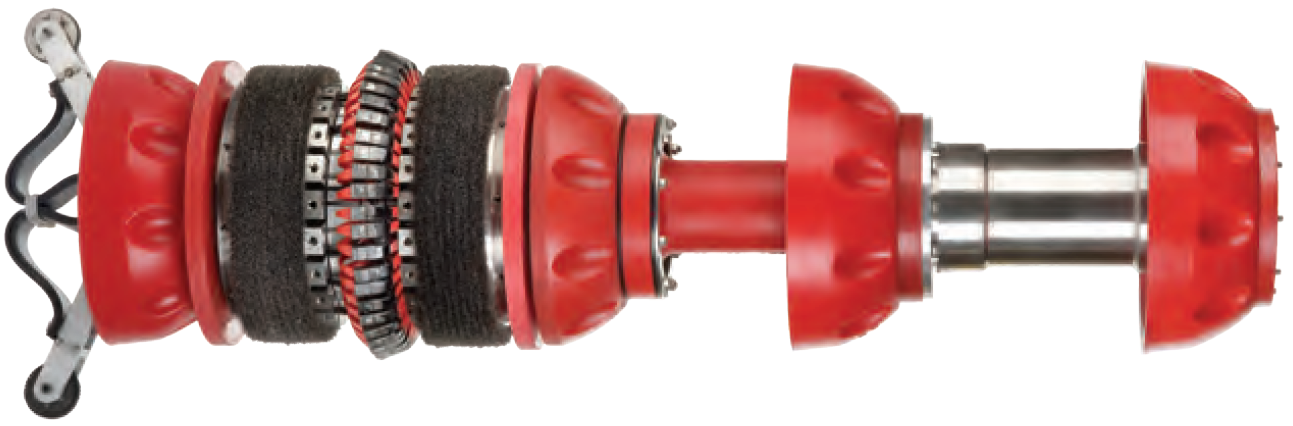
\includegraphics[width=.6\textwidth]{fig/pig/smartpig}
	\caption{Scovolo a dispersione di flusso magnetico \parencite{williamson2015guide}.}
	\label{fig:smartpig}
\end{figure}

La ricerca nel settore degli scovoli intelligenti è molto attiva e le soluzioni in commercio sono innumerevoli. Fra queste troviamo i \textit{pig} a neutroni, utili per rilevare nelle condotte sottomarine le sezioni non più sotterrate (\textit{span}). Le aree a contatto con l'acqua sono soggette a maggiori fenomeni di danneggiamento. 
%Nella pratica comune vengono impiegati degli strumenti esterni per rilevare degli \textit{span} attraverso lo scovolo a neutroni si riducono il numero di indagini e si migliora l'accuratezza dell'analisi.\\
Gli \textit{span} possono essere rilevati da strumenti esterni alla condotta; attraverso lo scovolo a neutroni si riducono il numero di indagini e si migliora l'accuratezza dell'analisi.\\
Altri esempi includono delle videocamere montate sullo scovolo, impiegate per l'ispezione interna visuale oppure scovoli per il rilevamento di curvature in condotte nelle aree artiche, corrispondenti a sollecitazioni locali causate dalle differenze di temperatura.

\subsection{Scovoli gel}
In questo caso non si parla di dispositivi di forma propria, bensì di sistemi a base di liquidi gelificati (\figref{fig:gelpig}) che sono sviluppati per le operazioni ausiliare in condotta come avvio della produzione, operazioni di supporto agli scovoli tradizionali o programmi di mantenimento.\\
La maggior parte dei gel impiegati sono a base di acqua, tuttavia possono essere anche a base di glicol, metanolo o altre sostanze liquida a seconda delle esigenze tecniche.\\
I tipi di scovoli gel disponibili sono:
\begin{itemize}
	\item \textbf{gel di \textit{batching}};
	\item \textbf{gel per cattura di detriti};
	\item \textbf{idrocarburi gelificati};
	\item \textbf{gel disisdratanti}
\end{itemize}

I principi applicativi degli scovoli gel vanno dalla separazioni delle diverse fasi liquide alla rimozione dei detriti, dai test di riempimento condotta allo spiazzamento dei liquidi indesiderati, fino all'impiego di sostanze chimiche come inibitori o biocidi. Importante sottolineare l'impiego del gel nello sblocco di scovoli tradizionali incastrati in condotta.

\begin{figure}[htbp]
	\centering
	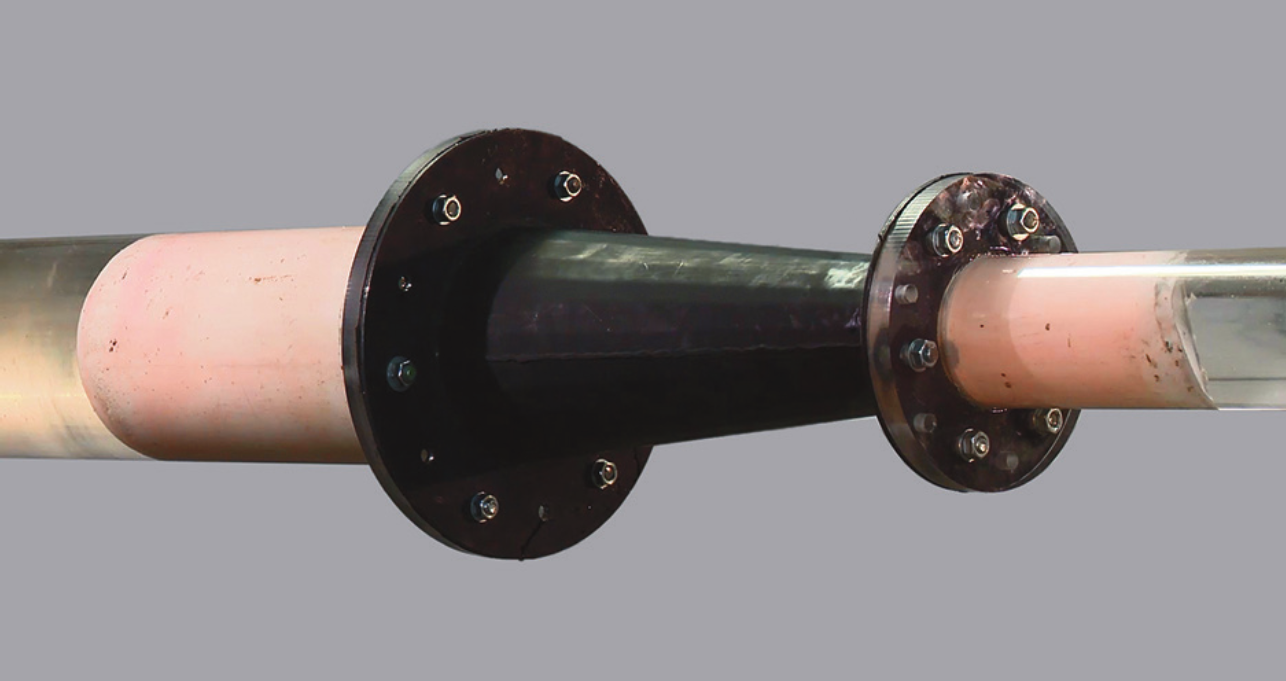
\includegraphics[width=.7\textwidth]{fig/pig/gelpig}
	\caption{Scovolo gel EVO-Pig, Aubin Ltd \parencite{johnston2015breaking}.}
	\label{fig:gelpig}
\end{figure}


%-------------------------------------------------------------------

\section{Procedure di lancio e recupero del pig}
Gli scovoli possono essere inseriti direttamente in condotta tramite dispositivi a spola. Tuttavia l'immissione e il recupero del \textit{pig} in condotta viene effettuata di norma tramite trappole di lancio e di ricezione. La scelta delle trappole di lancio e di ricezione dipende da numerosi fattori.\\
Le trappole sottomarine e quelle su terraferma hanno configurazione diversa. Si richiedono inoltre dispositivi di sicurezza addizionali al fine di garantire la sicurezza nelle operazioni. Dal rispetto della sequenza operativa nell'apertura e chiusura delle valvole della trappola dipende la probabilità di successo dell'applicazione: un'errata apertura o regolazione di una valvola può portare al blocco dello scovolo in condotta.\\
Le tipologia e la dimensione dello scovolo condizionano la scelta di una trappola di lancio o di ricezione. Nel caso di impiego di sfere le trappole possono essere più corte rispetto a quelle dedicate agli scovoli a mandrino. Al contrario, con l'impiego di scovoli intelligenti, la lunghezza richiesta aumenta notevolmente.\\
In molti casi le operazioni di piggaggio avvengono con il lancio di più scovoli contemporaneamente: ciò prevede l'utilizzo di organi di lancio e ricezione che possano contenere tutte le unità immesse nella condotta, aumentando così la lunghezza richiesta per la trappola.\\
Le trappole possono essere installate in modo permanente o temporaneo. In questo caso la configurazione cambia in modo sostanziale, così come i dispositivi di chiusura. Le trappole temporanee possono avere una chiusura semplice a flange, le trappole permanenti tendono a prediligere l'utilizzo di portelloni di chiusura rapida (\figref{fig:chiusuratrappola}).
\begin{figure}[htbp]
    \centering
    \subfloat[][Chiusura a anello con morsetto.]
    {\makebox[0.45\textwidth]{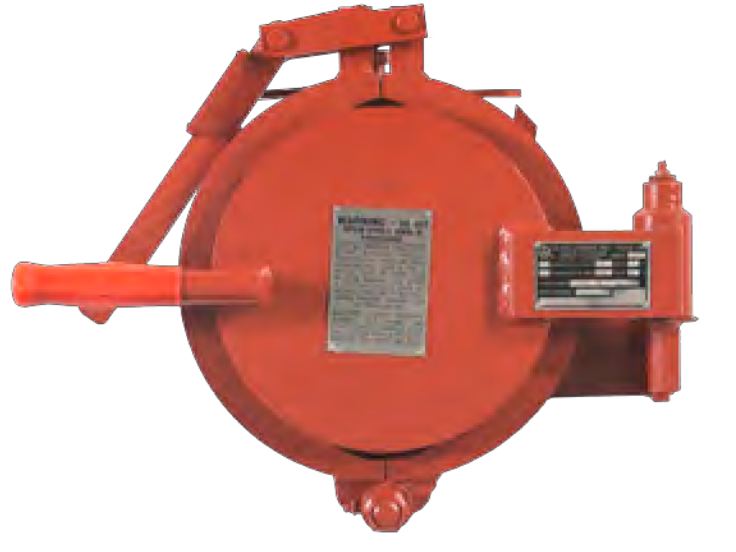
\includegraphics[width=.3\textwidth]{fig/pig/chiusura/anellomorsetto}}  \label{fig:anellomorsetto}} \qquad
    \subfloat[][Chiusura con rivestimento filettato.]
    {\makebox[0.45\textwidth]{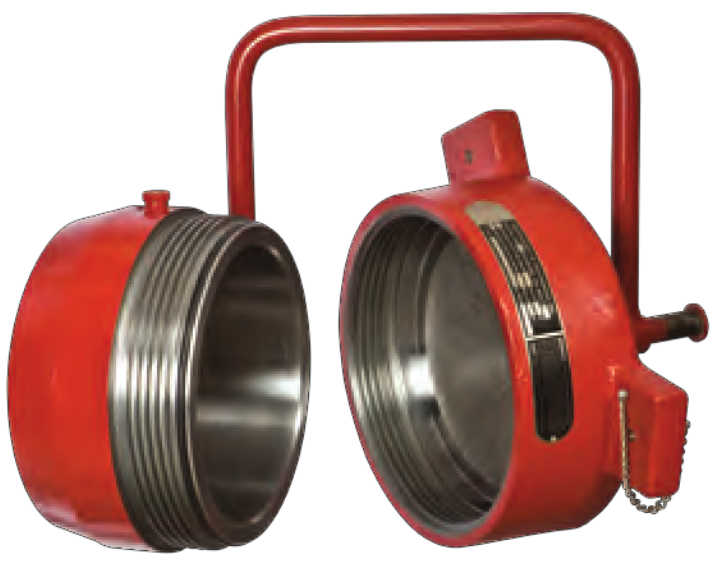
\includegraphics[width=.3\textwidth]{fig/pig/chiusura/filettato}}  \label{fig:filettato}}
\caption{Dispositivi di chiusura a portelloni delle trappole di lancio e ricezione \parencite{williamson2015guide}.}
\label{fig:chiusuratrappola}
\end{figure}

La configurazione della trappola si adatta al metodo di lancio degli scovoli in condotta. Un treno di più \textit{pig} può essere lanciato assieme oppure individualmente a intervalli stabiliti, interrompendo più volte il flusso del fluido di spinta per inserire un nuovo scovolo. Lo stesso scovolo può essere introdotto senza interrompere la produzione, pareggiando di volta in volta le condizioni di pressione della trappola con la condotta interessata.\\
Una tipica trappola di lancio (\figref{fig:piglauncher}), a prescindere dalla configurazione, prevede sempre l'installazione di determinate valvole.
La valvola di \textit{bypass} (\textit{mainline bypass valve}) regola il passaggio del flusso per la trappola o meno.
La valvola di ventilazione (\textit{vent valve}) consente la regolazione della pressione nella trappola, la depressurizzazione per l'inserimento dello scovolo in sicurezza e di nuovo la pressurizzazione.
La valvola di drenaggio (\textit{drain valve}) è utile al drenaggio per gravità del liquido all'interno della trappola.
La valvola di piggaggio (\textit{pigging valve}) mantiene lo scovolo all'interno della trappola fino alla sua apertura. 
La valvola di \textit{kick} (\textit{trap kicker valve}) conferisce allo scovolo la spinta idraulica necessaria per scorrere nella condotta.

\begin{figure}[htbp]
	\centering
	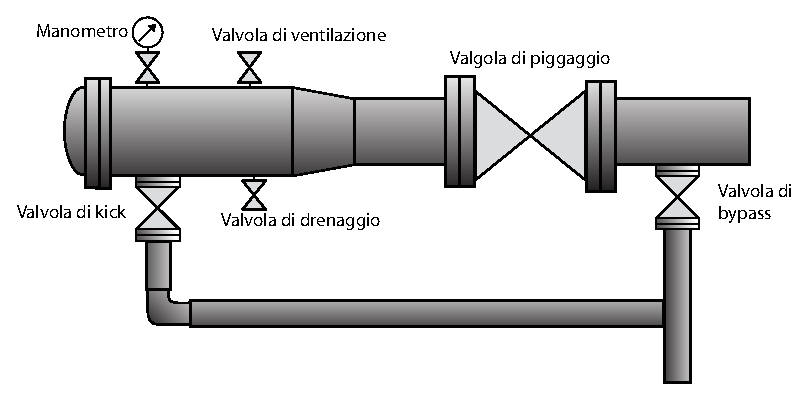
\includegraphics[width=.8\textwidth]{fig/pig/launcher.eps}
	\caption{Configurazione base di una trappola di lancio \parencite{davidson2002introduction}.}
	\label{fig:piglauncher}
\end{figure}

Le trappole di ricezione differiscono non di molto dai sistemi di lancio. La differenza sostanziale risiede nella lunghezza della trappola e la collocazione degli indicatori di posizione, necessari in entrambi i dispositivi per verificare l'avvenuto lancio o ricezione degli scovoli.

\subsection{Esempi di configurazione di sistemi di piggaggio}
Le trappole di lancio e di ricezione possono apparire simili nella configurazione, ma sul campo sono nettamente diversi per la variazione di geometria richiesta per le due applicazioni. I sistemi di piggaggio sono progettati per adattarsi alle specifiche della condotta e per svolgere diverse operazioni nel tempo. I sistemi di lancio/ricezione possono essere pensati in numerosi modi:
\begin{itemize}
\item \textbf{lancio verticale} (\figref{fig:launcher-verticale}): lancio di scovoli in posizione verticale, possibilità di automatizzare il processo;
\item \textbf{lancio standard del \textit{pig}} (\figref{fig:launcher-standard}): è possibile il lancio di un solo pig alla volta;
\item \textbf{lancio doppio o duale} (\figref{fig:launcher-duale}): combinazione di due trappole in parallelo su due condotte diverse, ma racchiuse in un unico sistema. Sistemi di questo tipo sono utilizzati dove si richiede il minore ingombro possibile, come in ambito \textit{off-shore};
\item \textbf{sistema di batch automatico} (\figref{fig:launcher-automatico-batch}): sistema automatizzato di lancio di treni di \textit{slug} interfacciati da degli scovoli di separazione;
\item \textbf{lancio inclinato} (\figref{fig:launcher-inclinato}): principio simile alle trappole verticali, la maggiore distanza di lancio consente un maggiore controllo dello scovolo in immissione;
\item \textbf{lancio combinato \textit{pig}/sfera} (\figref{fig:launcher-combo}): per esempio, nello spiazzamento dell'acqua tramite sfere e la deidratazione tramite scovoli a schiuma;
\item \textbf{sistemi di piggaggio automatico} (\figref{fig:launcher-automatico-pig}): sistemi totalmente automatizzati, capaci di inviare da remoto diversi tipi di scovolo (sfere, scovoli, etc.). Agli alti costi iniziali e operativi fa fronte l'alta efficienza delle applicazioni;
\item \textbf{sistemi di lancio per \textit{pig} di ispezione in linea} (\figref{fig:launcher-ispezione}): simili alle trappole convenzionali ma con camere di recupero molto più lunghe, per via delle dimensioni dello scovolo di ispezione interna.
\end{itemize}

\begin{figure}[htbp]
    \centering
    \subfloat[][Trappola di lancio verticale.]
    {\makebox[0.45\textwidth]{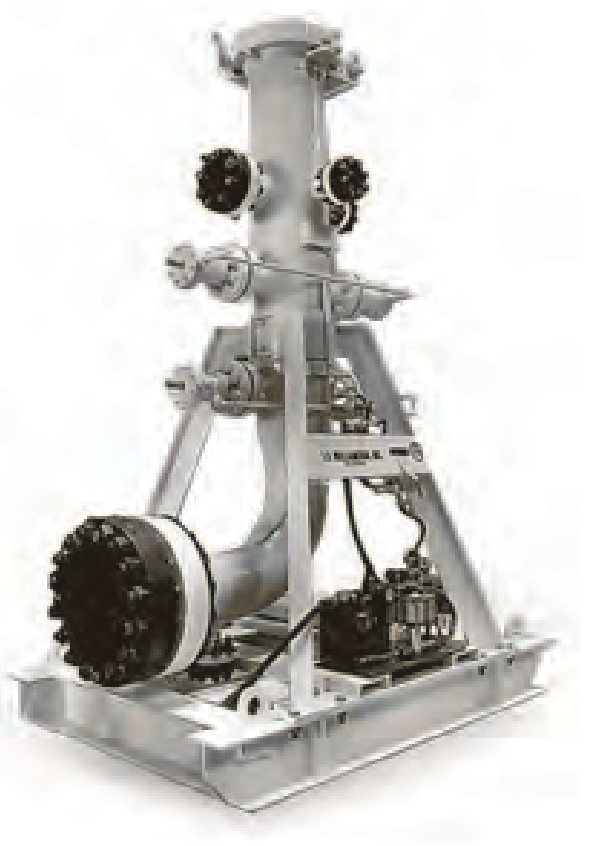
\includegraphics[height=.17\textheight]{fig/pig/launcher/verticale}}  \label{fig:launcher-verticale}}\qquad
    \subfloat[][Trappola di lancio standard.]
    {\makebox[0.45\textwidth]{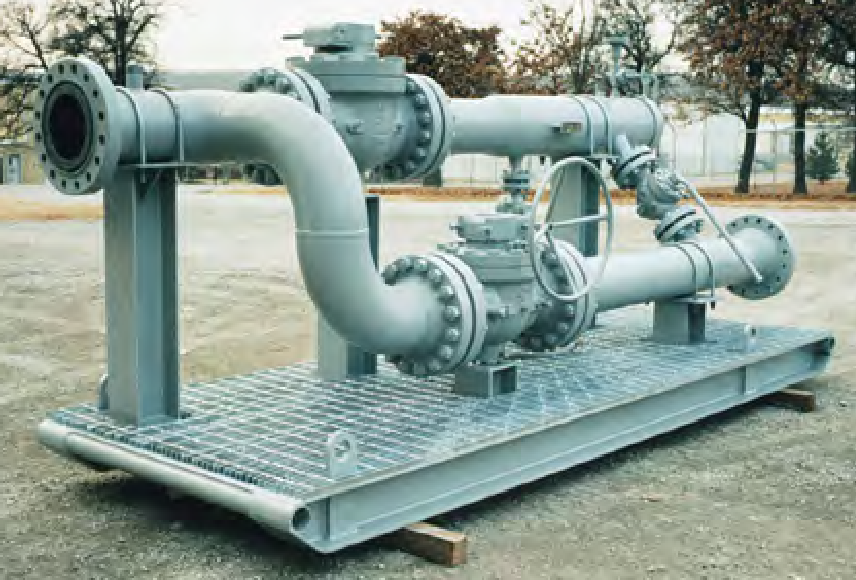
\includegraphics[height=.15\textheight]{fig/pig/launcher/standard}}  \label{fig:launcher-standard}}\\
    \subfloat[][Trappola di lancio duale.]
    {\makebox[0.45\textwidth]{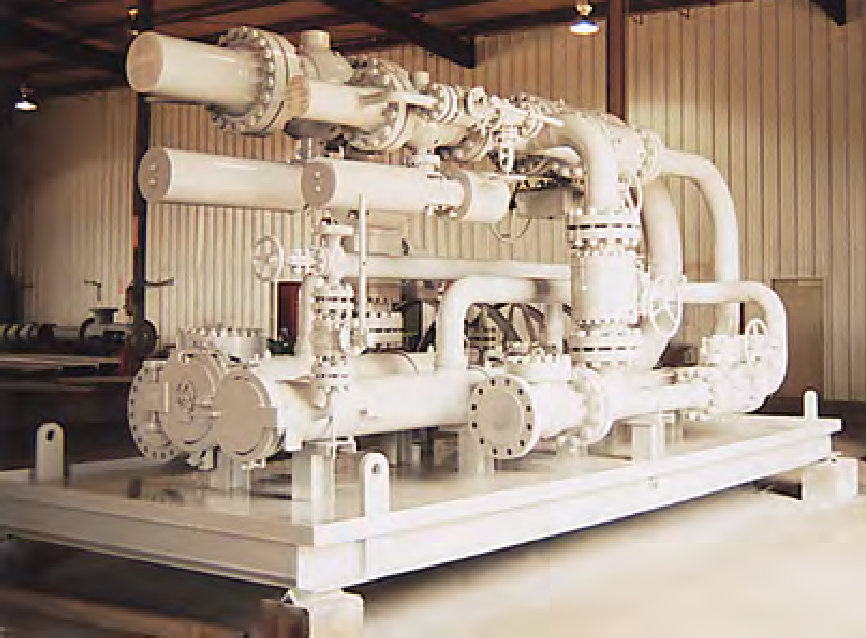
\includegraphics[height=.15\textheight]{fig/pig/launcher/duale}}  \label{fig:launcher-duale}}\qquad
    \subfloat[][Sistema di \textit{batching} in automatico.]
    {\makebox[0.45\textwidth]{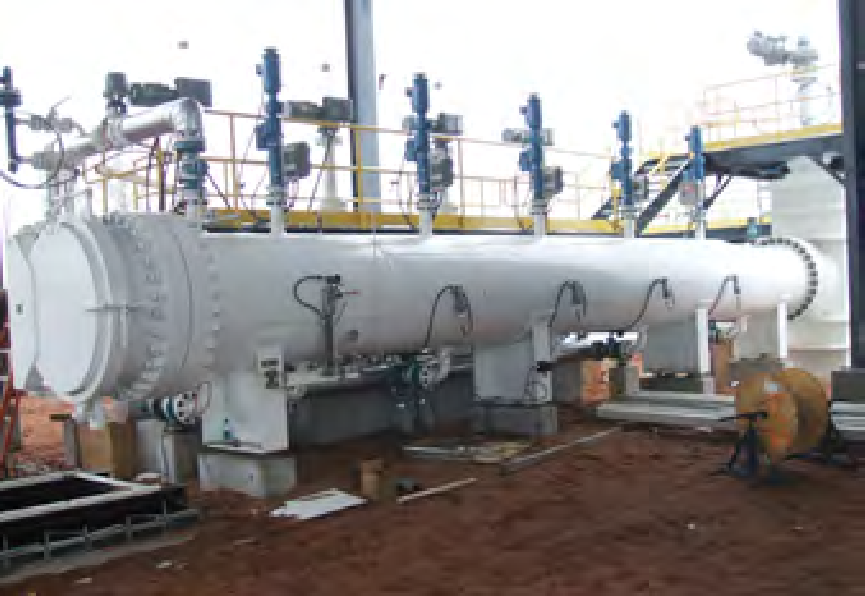
\includegraphics[height=.15\textheight]{fig/pig/launcher/automatico-batch}}  \label{fig:launcher-automatico-batch}}\\
    \subfloat[][Trappola di lancio inclinata.]
    {\makebox[0.45\textwidth]{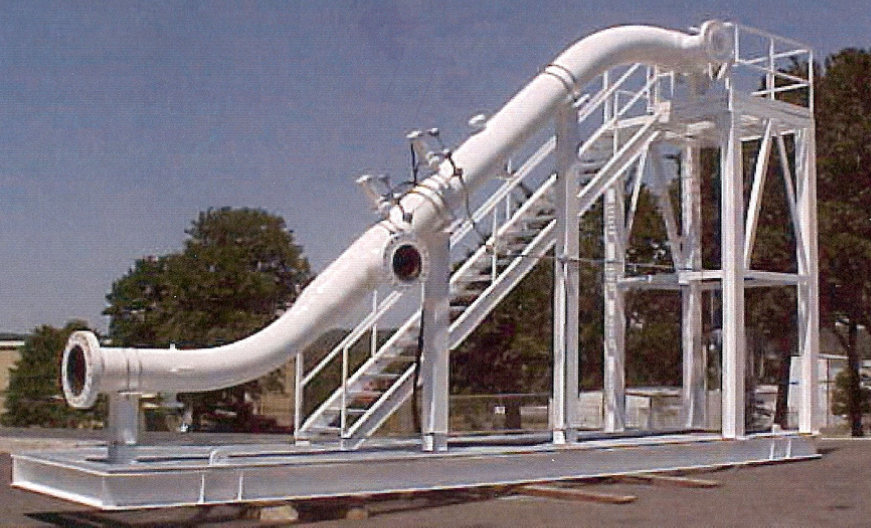
\includegraphics[height=.15\textheight]{fig/pig/launcher/inclinato}}  \label{fig:launcher-inclinato}}\qquad
    \subfloat[][Trappola per il lancio combinato scovolo/sfere.]
    {\makebox[0.45\textwidth]{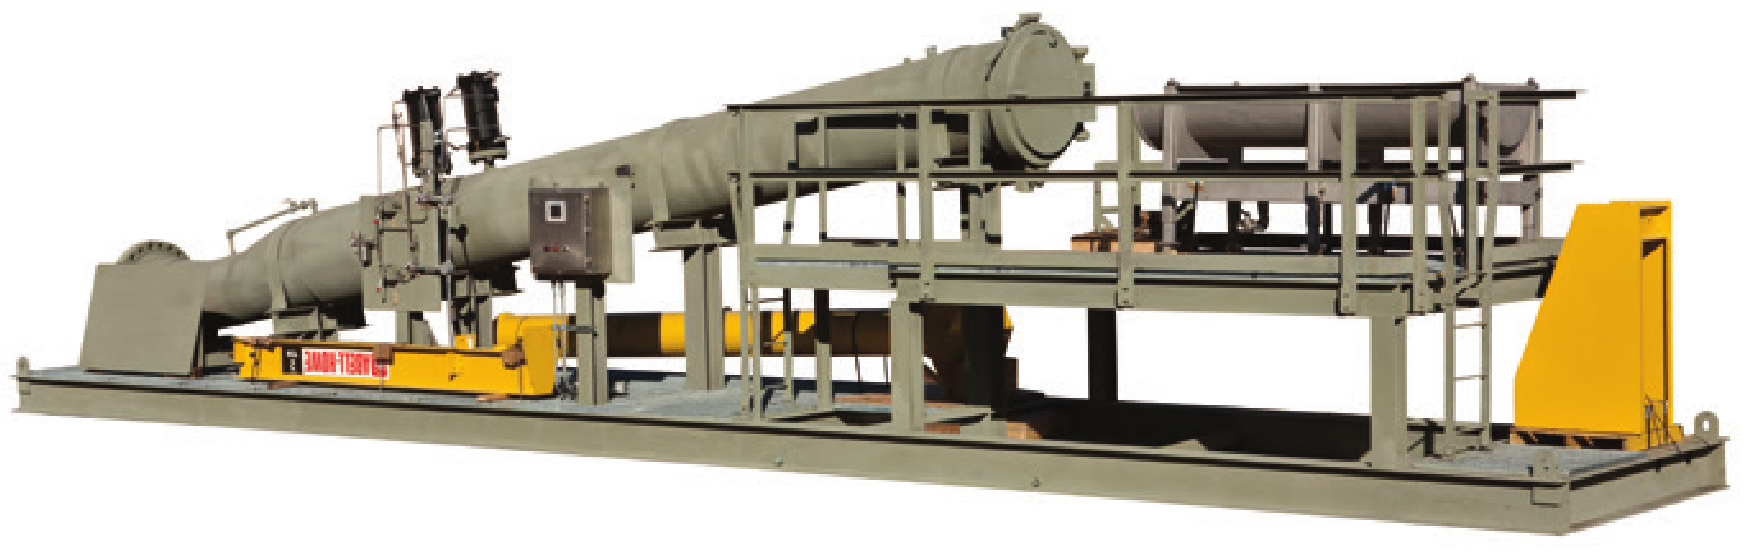
\includegraphics[height=.13\textheight]{fig/pig/launcher/combo}}  \label{fig:launcher-combo}}\\
    \subfloat[][Sistema di piggaggio automatico.]
    {\makebox[0.45\textwidth]{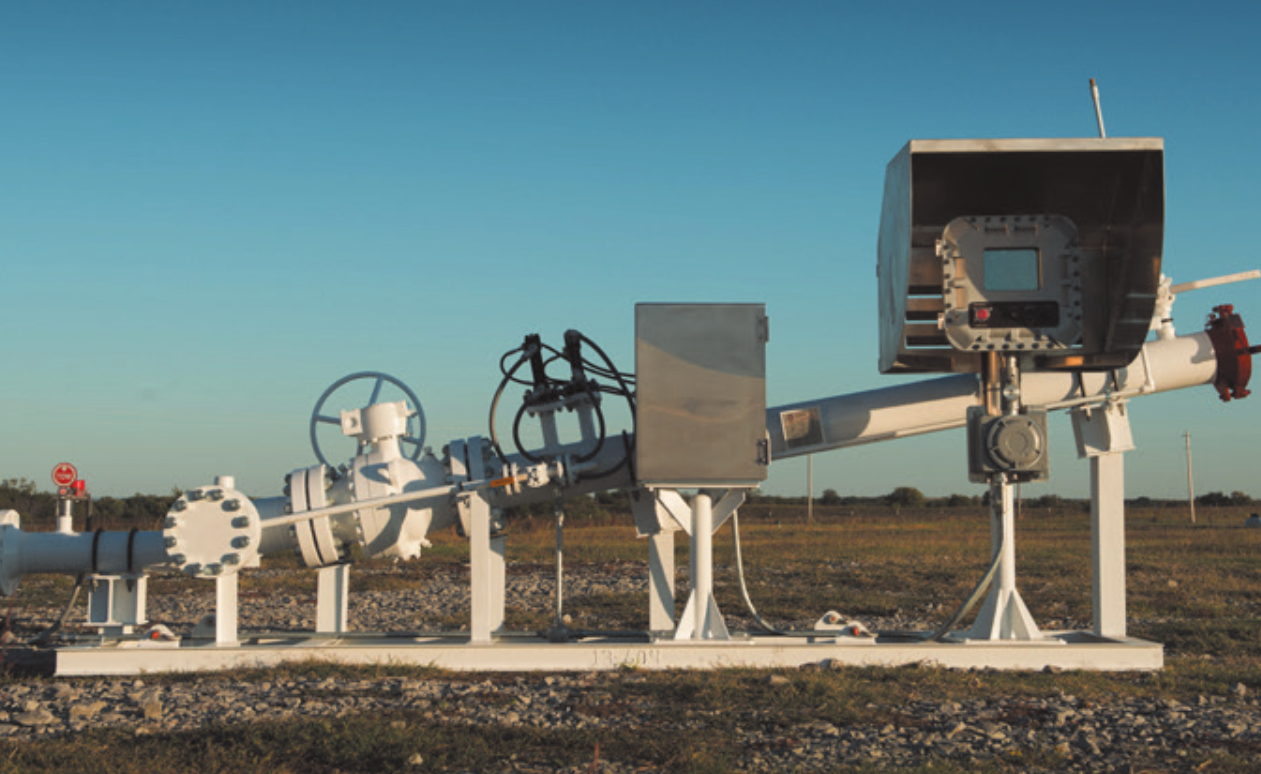
\includegraphics[height=.15\textheight]{fig/pig/launcher/automatico-pig}}  \label{fig:launcher-automatico-pig}}\qquad
    \subfloat[][Trappola di lancio per ispezione in linea.]
    {\makebox[0.45\textwidth]{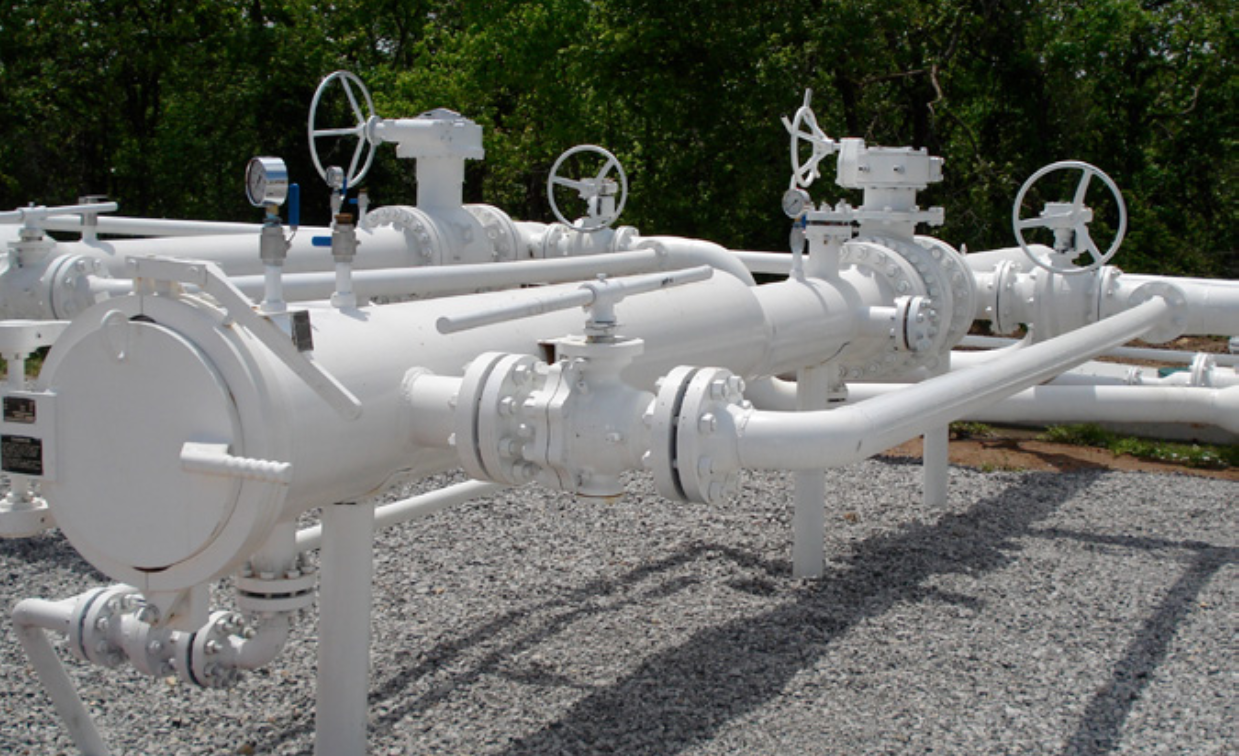
\includegraphics[height=.15\textheight]{fig/pig/launcher/ispezione}}  \label{fig:launcher-ispezione}}\\
\caption{Diverse tipologie di trappole di lancio \parencite{williamson2015guide}.}
\label{fig:launcher-tipologie}
\end{figure}
%--------------------------------------------------------------------------
\section{Mezzo di spinta del piggaggio}
In linea di massima si preferisce sospingere lo scovolo tramite un fluido incomprimibile. I liquidi incomprimibili consentono un maggiore controllo della velocità del \textit{pig} e minore usura delle guarnizioni, ottimizzando quindi l'efficacia e la tenuta idraulica dello strumento. Liquidi come acqua, olio o prodotti chimici e di processo possono essere utilizzati come mezzi di spinta. Gli organi di tenuta idraulica devono essere idonei con l'utilizzo di tale mezzo liquido.\\
I gas, essendo comprimibili, acquistano notevole energia in forma di pressioni prima che lo scovolo cominci a scorrere lungo la condotta. L'impiego di mezzi gassosi deve tenere conto di questi aumenti di pressione in condotta. Un apporto non sufficiente di gas, quindi una pressione non adeguata a monte dello scovolo,  può generare un movimento del dispositivo a scatti (\textit{stop-start motion}). L'effetto può essere attenuato con il giusto dimensionamento e mantenendo la contropressione a monte costante al fine di mantenere la velocità dello scovolo costante. Quando si impiegano dei gas come mezzi di spinta, è importare ricordare un possibile aumento dell'usura degli organi di tenuta. \\
Quando il mezzo di spinta consiste in un fluido multifase, si devono tenere in considerazione gli aspetti legati ai mezzi comprimibili e incomprimibili. L'impiego di più fasi possono generare flussi a \textit{slug} e le condotte, così come le trappole, devono essere progettate per questa applicazione (e.g. installazione di \textit{slug catcher} in prossimità della trappola di ricezione).

%--------------------------------------------------------------------------

\section{Progettazione del sistema di condotte per il piggaggio}
Il sistema deve essere progettato in modo tale da evitare imprevisti nelle operazioni di piggaggio. Di conseguenza ci sono degli importanti elementi di design da tenere in considerazione.
\subsection{Lunghezza del cammino del pig}
La distanza tra le varie trappole dislocate su una linea è determinata dalla lunghezza della condotta e dalla possibilità di installazione degli organi di lancio e di ricezione. La distanza massima percorribile da uno scovolo dipende dal tipo di mezzo di spinta dello scovolo:
\begin{itemize}
    \item 160 km per linee a gas;
    \item 240 km per linee di produzione (multifase);
    \item 320 km per linee a olio.
\end{itemize}
Le distanze massime percorribili dallo scovolo sono riferite non allo spostamento fisico, bensì al percorso massimo con livelli minimi di efficacia del piggaggio. Come già detto in precedenza le linee a gas sono molto più abrasive e tendono a consumare più velocemente gli organi di tenuta. Le linee a olio offrono una lubrificazione naturale del dispositivo, garantendo una distanza doppia rispetto a quelle a gas.

\subsection{Raggio di curvatura}
Ogni scovolo è progettato per attraversare determinati raggi di curvatura minimi della condotta. Assieme al raggio di curvatura si fa riferimento all'angolo di curvatura, riferito al cambio di direzione della linea. In questo ambito i raggi di curvatura sono espressi in R/D, rapporto tra il raggio di curvatura e il diametro nominale della condotta. Solitamente si fa riferimento a 1,5 R/D per condotte a gas, 3 R/D per condotte a olio e 1 R/D per piccole condotte di raffineria.
\subsection{Tipologia di valvole presenti}
Le valvole a sfera moderne, o rubinetti sferici, garantiscono il passaggio degli scovoli lungo la linea. In presenza però di rubinetti sferici di vecchia generazione, quindi non progettati per il piggaggio della condotta, può accadere il blocco del dispositivo (\figref{fig:pig-rubinettosfera}). Al fine di prevenire il blocco deve essere tenuta in stretta considerazione la dimensione della sede della valvola in rapporto alla lunghezza dello scovolo.\\
In presenza di valvole di ritegno, lo scovolo deve essere abbastanza grande da oltrepassare la valvola e mantenerla completamente aperta. Scovoli e sfere troppo piccole possono permanere nella sede della valvola, mantenendola aperta e bypassando di fatto il dispositivo (\figref{fig:pig-nonritorno}).
\begin{figure}[htbp]
    \centering
    \subfloat[][Blocco dello scovolo in valvola a sfera.]
    {\makebox[0.4\textwidth]{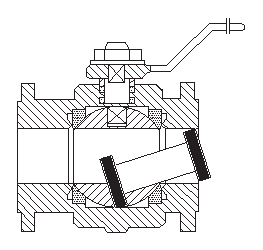
\includegraphics[height=.22\textheight]{fig/pig/rubinettosfera.eps}}  \label{fig:pig-rubinettosfera}}\qquad
    \subfloat[][Blocco della sfera in valvola di ritegno.]
    {\makebox[0.4\textwidth]{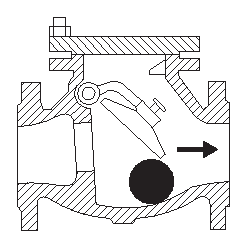
\includegraphics[height=.2\textheight]{fig/pig/nonritorno.eps}}  \label{fig:pig-nonritorno}}\\
    \caption{Blocco degli scovoli in corrispondenza di valvole \parencite{guadagni2003prontuario}.}
    \label{fig:piggaggio-valvole}
\end{figure}

\subsection{Indicatori di passaggio del pig}
Gli indicatori di passaggio dello scovolo sono utilizzati per rilevare l'attraversamento del \textit{pig} per un determinato punto della condotta, oppure per verificare l'avvenuto lancio o ricezione. Gli indicatori sono importanti nei sistemi automatizzati di piggaggio poiché sono collegati alle valvole e alle stazioni di pompaggio, le quali si attivano una volta giunto lo scovolo in posizione.

\begin{figure}[htbp]
    \centering
    \subfloat[][Indicatore di posizione a bandierina.]
    {\makebox[0.45\textwidth]{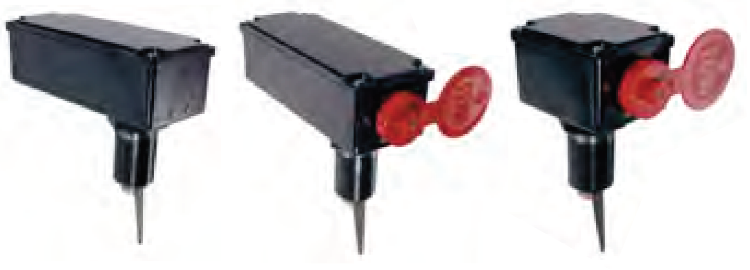
\includegraphics[height=.10\textheight]{fig/pig/indicatori/passaggio}}  \label{fig:indicatori-passaggio}}\qquad
    \subfloat[][Indicatori di posizione elettronici a bandierina.]
    {\makebox[0.45\textwidth]{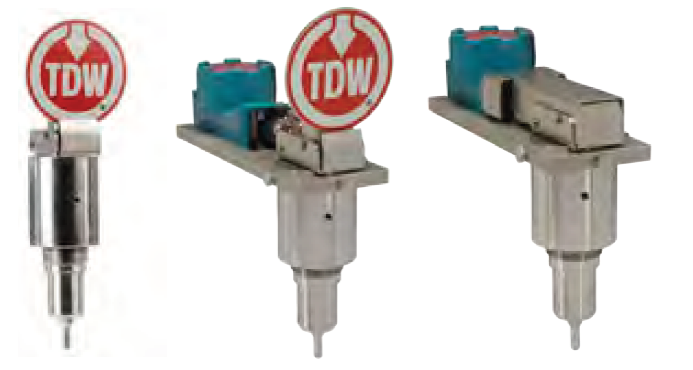
\includegraphics[height=.10\textheight]{fig/pig/indicatori/elettrici}}  \label{fig:indicatori-elettrici}}\\
    \subfloat[][Indicatore di posizione magnetico.]
    {\makebox[0.45\textwidth]{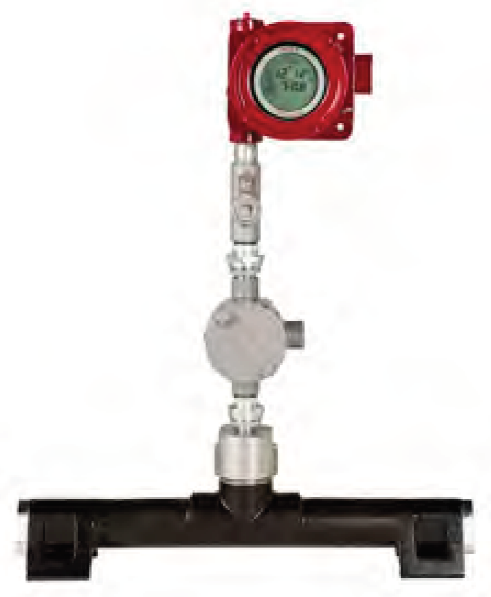
\includegraphics[height=.17\textheight]{fig/pig/indicatori/magnetici}}  \label{fig:indicatori-magnetici}}
    \caption{Indicatori di posizione dello scovolo in condotta \parencite{williamson2015guide}.}
    \label{fig:indicatori-piggaggio}
\end{figure}

\subsection{Altri dettagli progettuali}
I raccordi a T (\textit{tee}), la cui condotta di ingresso supera la metà del diametro della condotta principale, richiedono l'installazione di guide, al fine di prevenire il bloccaggio dello scovolo. Le guide possono essere di varia natura, come \textit{coupon} o \textit{tee barred}. Inoltre si evitano l'installazione di raccordi a T adiacenti l'un l'altro.\\
Le condotte laterali possono essere installate, lo scovolo in questo caso deve avere lunghezza superiore alla sede di immissione della condotta.\\
Variazioni drastiche del diametro interno vanno evitate. Lo scovolo deve essere adatto alle variazioni di dimensione interna e deve garantire la tenuta in tutte le sezioni interessate dal piggaggio. La stessa considerazione deve essere effettuata per linee costituite da condotte con diametro nominale diverso. 

\section{Bloccaggio dello scovolo}
Il piggaggio presenta in generale determinati rischi: a prescindere dalle precauzioni prese, esiste sempre una minima probabilità che questo evento accada. Il blocco dello scovolo in condotta (\textit{stuck pig}) può creare ostruzione completa (\textit{full stuck pig}) interrompendo la produzione e causando notevoli danni. La chiusura può essere parziale (scovolo in \textit{bypass}): le conseguenze non sono immediate e occorre in ogni modo rimuovere il dispositivo incastrato in condotta.\\
La condizione di \textit{stuck pig} è caratterizzata da bassa frequenza dell'evento, cause difficilmente identificabili e al peggioramento delle condizioni iniziali in caso di una soluzione non idonea.\\
In caso di blocco dello scovolo si devono limitare azioni impulsive, individuare la soluzione finale certa per la risoluzione del problema, pianificare diversi tentativi per comprendere la soluzione migliore in termine di tempi e costi.
\subsection{Soluzioni}
Ogni possibile soluzione da adottare richiede delle condizioni al contorno da soddisfare, delle precise procedure e sequenze operative da seguire e degli effetti, cioè le conseguenze che l'applicazione può apportare. Le soluzioni possono essere classificate in:
\begin{itemize}
	\item \textbf{preliminari}: verifica della situazione e dello stato del problema;
	\item \textbf{di tentativo}: la soluzione può risolvere o meno il blocco;
	\item \textbf{di localizzazione}: per comprendere la posizione dello scovolo, a volte possono portare allo sblocco non programmato;
	\item \textbf{meccaniche}: interventi meccanici puntuali sulla tubazione o su un tratto più o meno esteso;
	\item \textbf{ausiliarie}: tentativo di mitigazione del problema (e.g. passaggio dalla condizione di \textit{full stuck pig} a quella di scovolo in \textit{bypass}).
\end{itemize}

\subsection{Fasi operative}
Il primo step per l'analisi della procedura di sblocco più idonea prevede la raccolta dei dati inerenti le condizioni di impianto, le caratteristiche del fluido e dello scovolo. Conoscendo le condizioni al contorno iniziali si scartano le soluzioni non applicabili nel determinato contesto\\
Il secondo step consiste nella valutazione delle diverse soluzioni possibili, valutando quella che minimizza tempi e costi. Questa soluzione di riferimento sarà l'elemento base per l'elaborazione delle alternative possibili. \'E importante comprendere le probabilità di insuccesso e gli effetti negativi associati alla soluzione di riferimento, utile alla formulazione di una stima dei tempi e costi della procedura di sblocco.\\
Dalla soluzione di riferimento si esaminano tutte le soluzioni di tentativo che possano aumentare la probabilità di riuscita della procedura. Alcune soluzioni di tentativo possono portare all'effetto opposto, sancendo l'inapplicabilità della soluzione di riferimento.\\
Una volta prese in considerazione le soluzioni di tentativo e quella di riferimento, si studiano nel complesso le varie combinazioni in sequenza temporale e si comprende quale successione possa avere più probabilità di successo. Le sequenze di soluzioni con un costo complessivo medio-basso rispetto alla soluzione di riferimento sono considerate valide alternative a quella principale.

\begin{figure}[htbp]
	\centering
	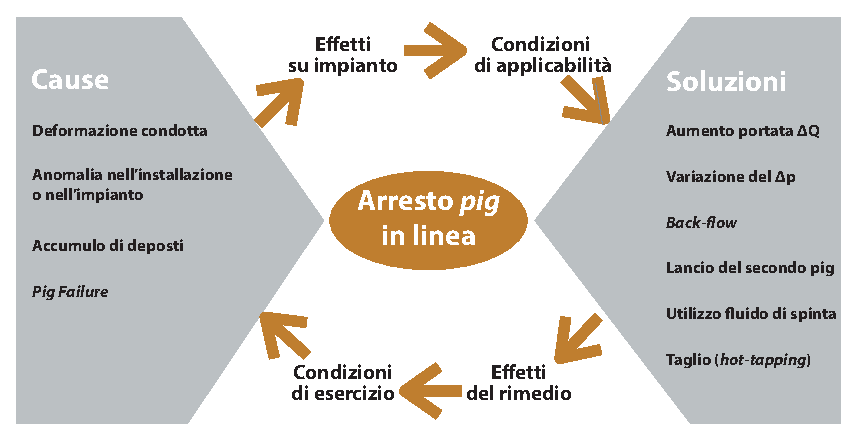
\includegraphics[width=\textwidth]{fig/pig/blocco.eps}
	\caption{Possibili cause e soluzioni legate all'arresto di \textit{pig} in linea \parencite{diluvio2006questione}.}
	\label{fig:bloccopig}
\end{figure}

Il piggaggio come soluzione di ripristino delle condizioni ottimali in condotta necessita di numerosi accorgimenti e la condotta deve essere predisposta allo scorrimento dello scovolo al suo interno. Il blocco dello scovolo in linea può portare a conseguenze importanti sull'impianto, oltre che all'interruzione della produzione. Molte volte la condotta non è piggabile a causa della configurazione della linea o alla bassa resistenza alle sollecitazioni meccaniche che l'applicazione può comportare. Una valida alternativa nell'ambito dello spiazzamento di liquidi in condotte a gas è rappresentata dall'impiego di tensioattivi in orizzontale: l'applicazione, seppur di recente realizzazione, sembra avere un'ottima efficacia ovviando ai problemi legati al piggaggio in linea.
